\section{Approximation error, verification and control}
\label{sec:examples}
We implemented the above smooth approximation to the semantics of MTL, and tested it empirically on a number of examples.

\subsection{Approximation error for robustness}
\label{sec: ex apx error}
\begin{figure}[t]
\centering
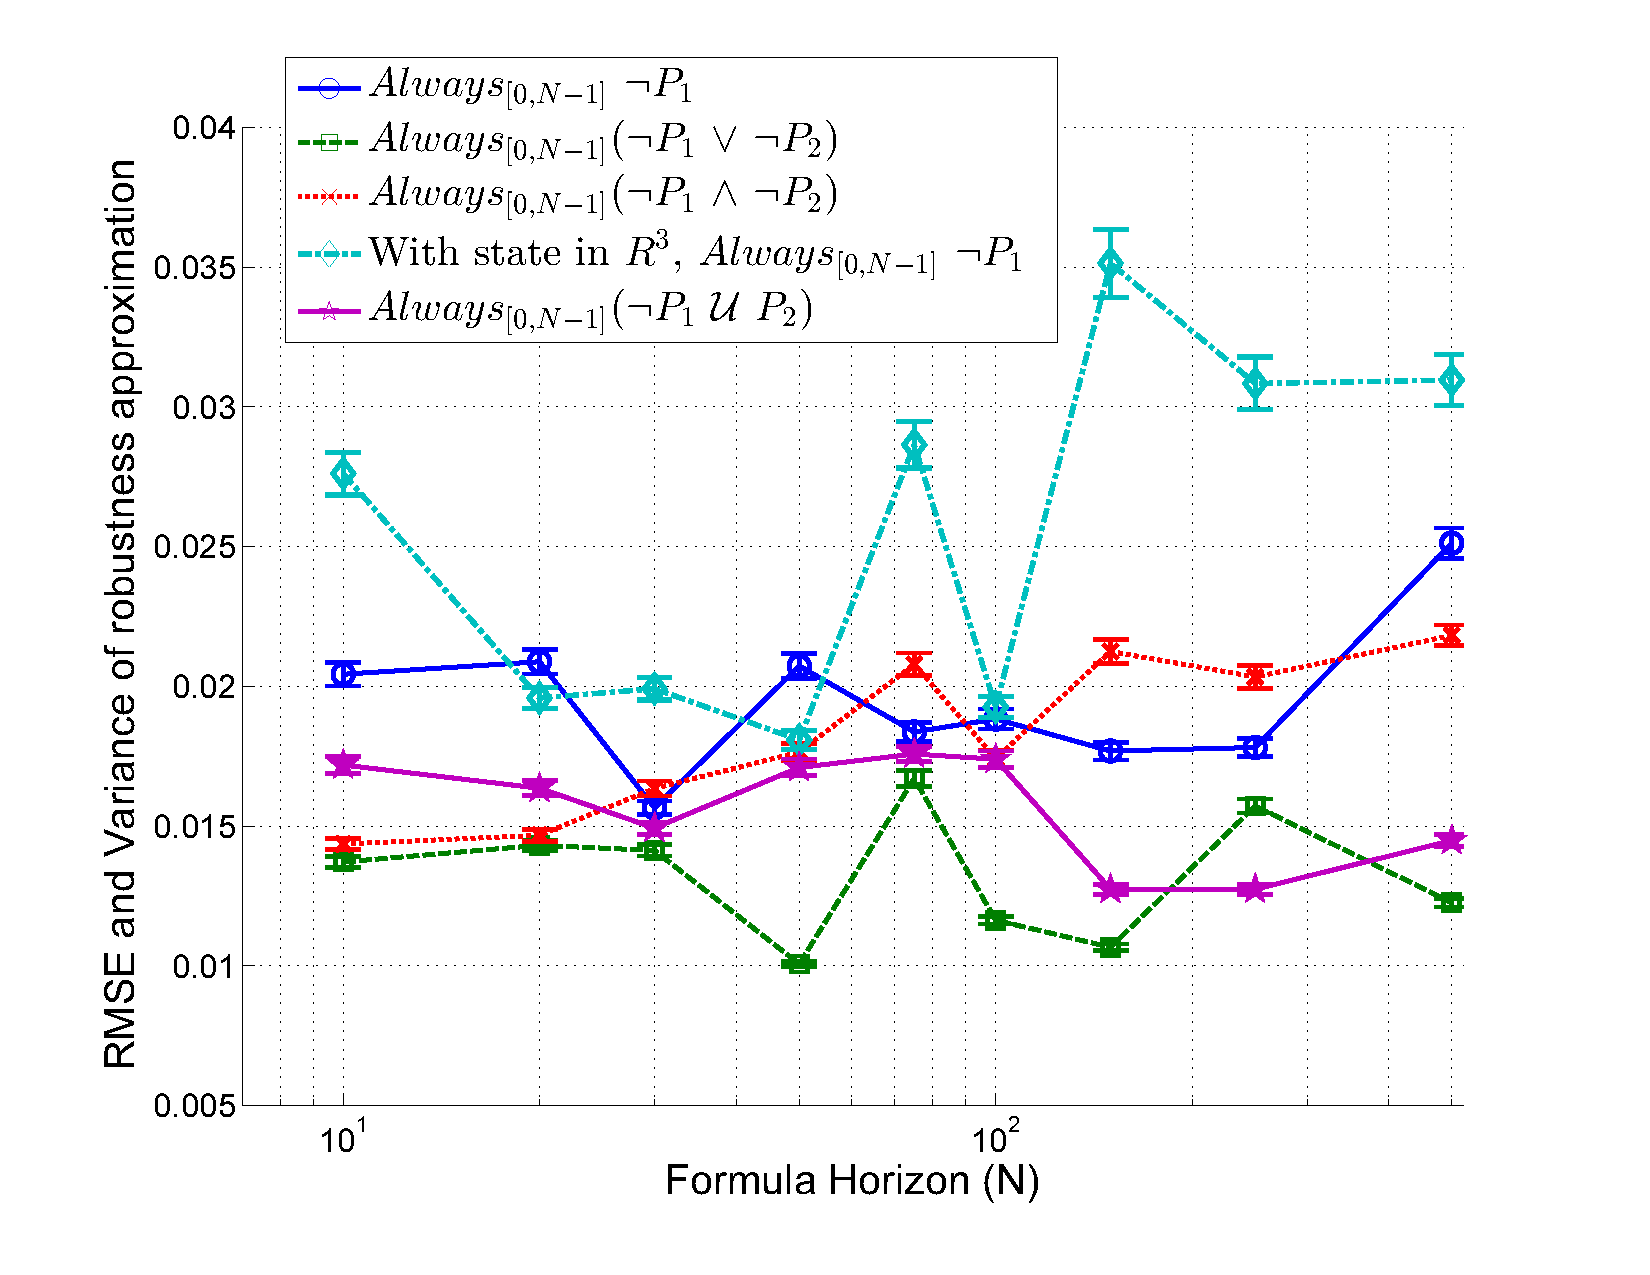
\includegraphics[width=0.49\textwidth]{figures/RobustnessError}
\vspace{-30pt}
\caption{{\small RMSE (and variance) of robustness approximation error against formula horizon, evaluated on 1000 randomly generated trajectories for the system in \eqref{eq:PointMass}. Unless noted, the states in the trajectory are in $\mathbb{R}^2$. Note, the magnitude of the approximation errors are very small, as is the variance, showing the accuracy of the smooth approximation of robustness.}}
\vspace{-10pt}
\label{fig:sample result}
\end{figure}

We evaluated the robustness $\robf$ and its approximation $\srobf$ for five formulae, with $hrz(\formula_i) = N$. $P_1$ and $P_2$ are atomic propositions for state being in two polyhedrons $P_1$ and $P_2$ respectively. 
%Each formula is of the form $\formula_i = \always_{[0:N-1]} \psi$, where $N$ is the length of the trajectory.
%Thus $hrz(\formula_i)  = N$.
Each formula's robustness is evaluated on 1000 randomly-generated trajectories of varying lengths $N$, so we can  examine the error's variation with the horizon.
The trajectories were produced by a 2-or-3 dimensional system, \eqref{eq:PointMass} with input and state saturation.
%All formulas use the atomic propositions $P_1 \defeq x \in [-1,1]^n$ and $P_2 \defeq x\in [2,2.5]^n$, where $n = 2,3$ is the dimension of the system.
%The state-space is $[-5,5]^n$ and the input set is $\inpSet = [-0.3,0.3]^n$. 

Fig. \ref{fig:sample result} shows the Root Mean Square (RMSE) of the approximation, $\sqrt{(1/1000)\sum_{\sstraj}(\robf(\sstraj)-\srobf(\sstraj))^2}$
, and variance bars around it. As seen, the approximation error is small for all cases.
As suggested by Remark \ref{rem:upper bound}, the approximation error generally increases with the horizon (for a constant number of wavelet coefficients).
This is due to the smooth max and min functions, as seen in \eqref{eq:smooth max error}.

%Fig. \ref{fig:relative error} shows the relative approximation errors, $(\robf-\srobf)/|\robf|$, for the formulae under consideration. 
%It is seen that the average relative approximation error is less than $10\%$ for all cases. 
%For some data points in Fig. \ref{fig:relative error}, the variance of relative error is high, but the error remains small in absolute terms as seen in Fig.~\ref{fig:sample result}.

%In general, the high relative approximation errors are due to trajectories which have a true robustness of near zero; 
%these lead to a spike in the relative approximation error, $(\robf-\srobf)/|\robf|$, even for small values of the absolute error $|\robf-\srobf|$.

%suggesting that the approximation errors vary wildly. This is not the case, as it is worth noting in Fig. \ref{fig:sample result} that the variance of the actual approximation is very small. 

%\todo[inline]{not sure what the point is in this paragraph...previous figure gives (roughly) average error. this gives relative error. one does not cancel out the other. the relative error does vary a lot in some case, as evidenced here. one can only say that even though relative error can vary a lot inn some case, the absolute }

Note that while the RMSE  increased with the system dimension ($4^{th}$ formula in Fig.~\ref{fig:sample result}), it was observed that the relative error remained very small i.e. the increase in error is explained by an increase in the robustness's magnitude. 
%As explained in the previous section, better approximation can be achieved by increasing the number of wavelet coefficients as dimension, and trajectory length, grow.
%\todo[inline]{Is that true?}

%\begin{figure}[t]
%\centering
%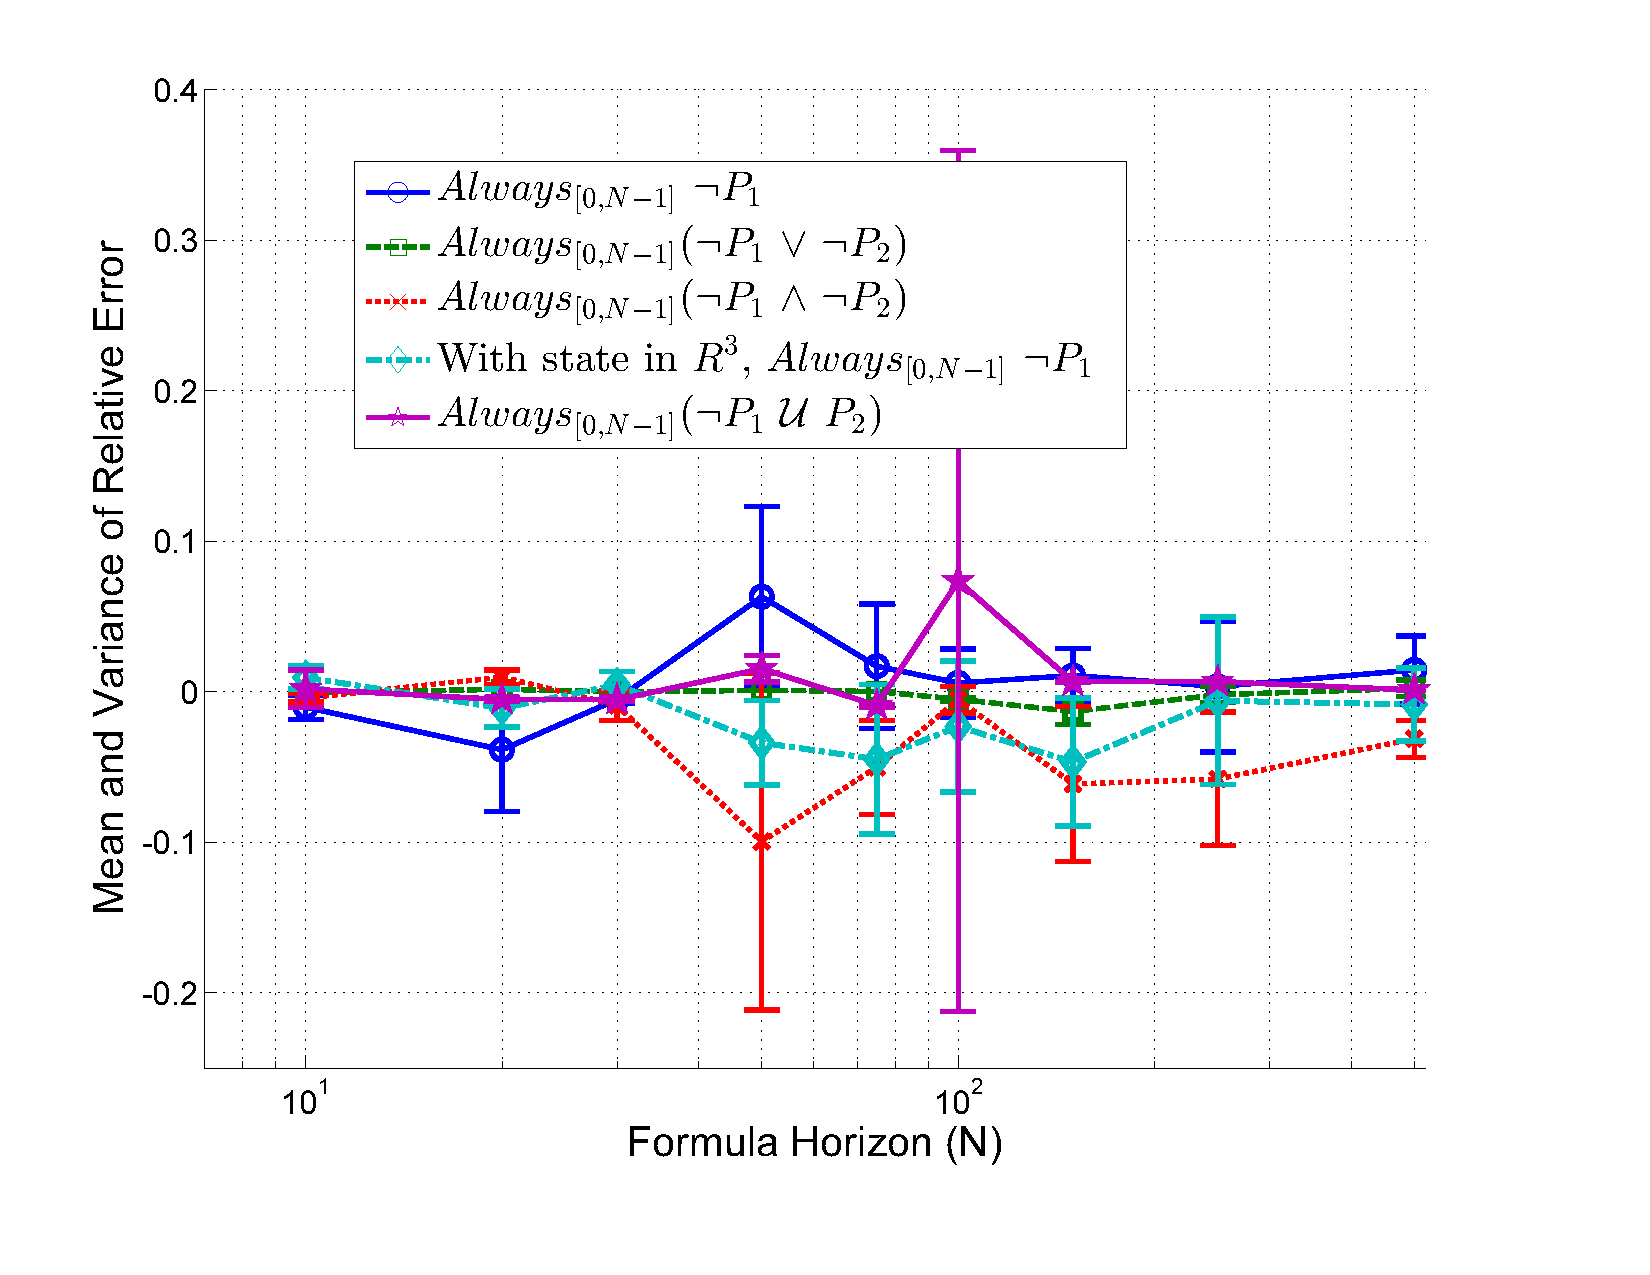
\includegraphics[width=0.49\textwidth]{figures/RobustnessErrorRel}
%\vspace{-30pt}
%\caption{{\small Mean and variance of relative approximation error against formula horizon, evaluated on 1000 randomly generated trajectories for the system in \eqref{eq:PointMass}. Unless noted, the states in the trajectory are in $\mathbb{R}^2$.}} 
%\todo[inline]{smae changes as previous fig. All temporal operators must be bounded}}
%\label{fig:relative error}
%\vspace{-15pt}
%\end{figure}

%\vspace{-30pt}
\subsection{Robustness maximization for control}
\label{sec:toy example}
%\todo[inline]{Yash, Show SA and SR-SQP on toy example}
%Toy example text
%\todo[inline]{I expect to see first the general control problem 13a-13e, then the specific example. This way, if you define once here, we dnot have to worry about re-defining the control problem later. So: here;s the general control problem; here's a simple system.}

The control problem we solve is a generalized version of \eqref{eq:min rob problem} (using the smooth version of robustness), given by
\begin{subequations}
\label{eq:general_ctrl}
\begin{align}
\text{max } & \srob_{\formula}(\sstraj) - \gamma \sum_{k=0}^{N-1} l(x_{k+1},u_{k}) \\
\text{s.t. } & x_{k+1} = f(x_k,u_k), \, \forall k=0,\dotsc,N-1 \\
 & x_k \in X, \, \forall k=0,\dotsc,N \\
 & u_k \in U, \, \forall k=0,\dotsc,N-1 \\
 & \delta \srob_{\formula}(\sstraj) \geq 0
\end{align}
\end{subequations}
%\todo[inline]{stick to $\formula$ for a formula, not $\formula$ (unless there's a good reason)}

If we set $\gamma=0$ and $\delta=0$, we recover the problem in \eqref{eq:min rob problem} with the smooth robustness in the cost function. In the above formulation, $l(x_{k+1},u_{k})$ is a system specific control cost, e.g. the LQR cost $x_k'Qx_k + u_k'Ru_k$. $X$ and $U$ define constraints on the state $x$ and control $u$ respectively. 

For illustrative purposes, we choose a simple linear system (point-mass dynamics) to first illustrate our method. The point-mass system has the following dynamics:
\begin{equation}
\label{eq:PointMass}
x_{k+1} = x_k + u_k
\end{equation}

For the point-mass example, we define the specification to be followed as $\formula = \always_{[0,20]} \neg (x_k \in \text{Unsafe}) \land \eventually_{[0,20]} (x_k \in \text{Terminal})$, with the sets $\text{Unsafe}=[-1,1]^2$ and $\text{Terminal}=[2,2.5]^2$. In addition, for the control problem, $X=[-2.5,2.5]^2$, $U=[0.3,0.3]^2$, $\delta=1$, and we optimize for two different values of $\gamma$, $0.1$ and $0.001$, and start with an initial point $x_0=[-2,-2]'$. The control cost is $l(x_k) = ||x_k||_{2}^2$, which when summed over is the square of the trajectory length. Note, $N=21$, which is the horizon length of the specification.

An initial trajectory starting from $x_0$ and ending in the $\text{Terminal}$ set is obtained via solving a linear program for feasibility with the system dynamics and input/state constraints, and the terminal set added as a constraint. This trajectory is used as an initial point to initialize the optimization.

We use MATLAB's Sequential Quadratic Programming (SQP) solver for the optimization, and also compute a gradient for $\srob$ to be used in SQP.
%\todo[inline]{confusing...you throw around things casually like $\min 0$, as if you're daring the reader to get confused. Or "This trajectory is used to initialize the SQP optimization, which is used for the optimization."..Take your time. explain it once, well, and then forget about it. this is the \textit{illustrative} example. see my comment in ATC case study.}
\todo[inline]{say a word or two about SQP: broadly, how it works and whether it has guarantees. after all, it is to use things like SQP that we are smoothing in the first place. }

Fig.~\ref{fig:toy control} shows the sets, initial trajectory (which is unsafe and has a robustness of $-1$), and the two trajectories for the two values of $\gamma$. Both trajectories satisfy the specification $\formula$. Intuitively, the trajectories in Fig.\ref{fig:toy control} make sense, as for a higher value of $\gamma=0.1$ we get a shorter trajectory, which is closer to unsafe set, hence satisfies $\formula$ less robustly ($\rob_{\formula}=0.6543$) and for a smaller value of $\gamma=0.001$ we get a longer trajectory which has a higher robustness ($\rob_{\formula}=1.2073$).

\begin{figure}[t]
\centering
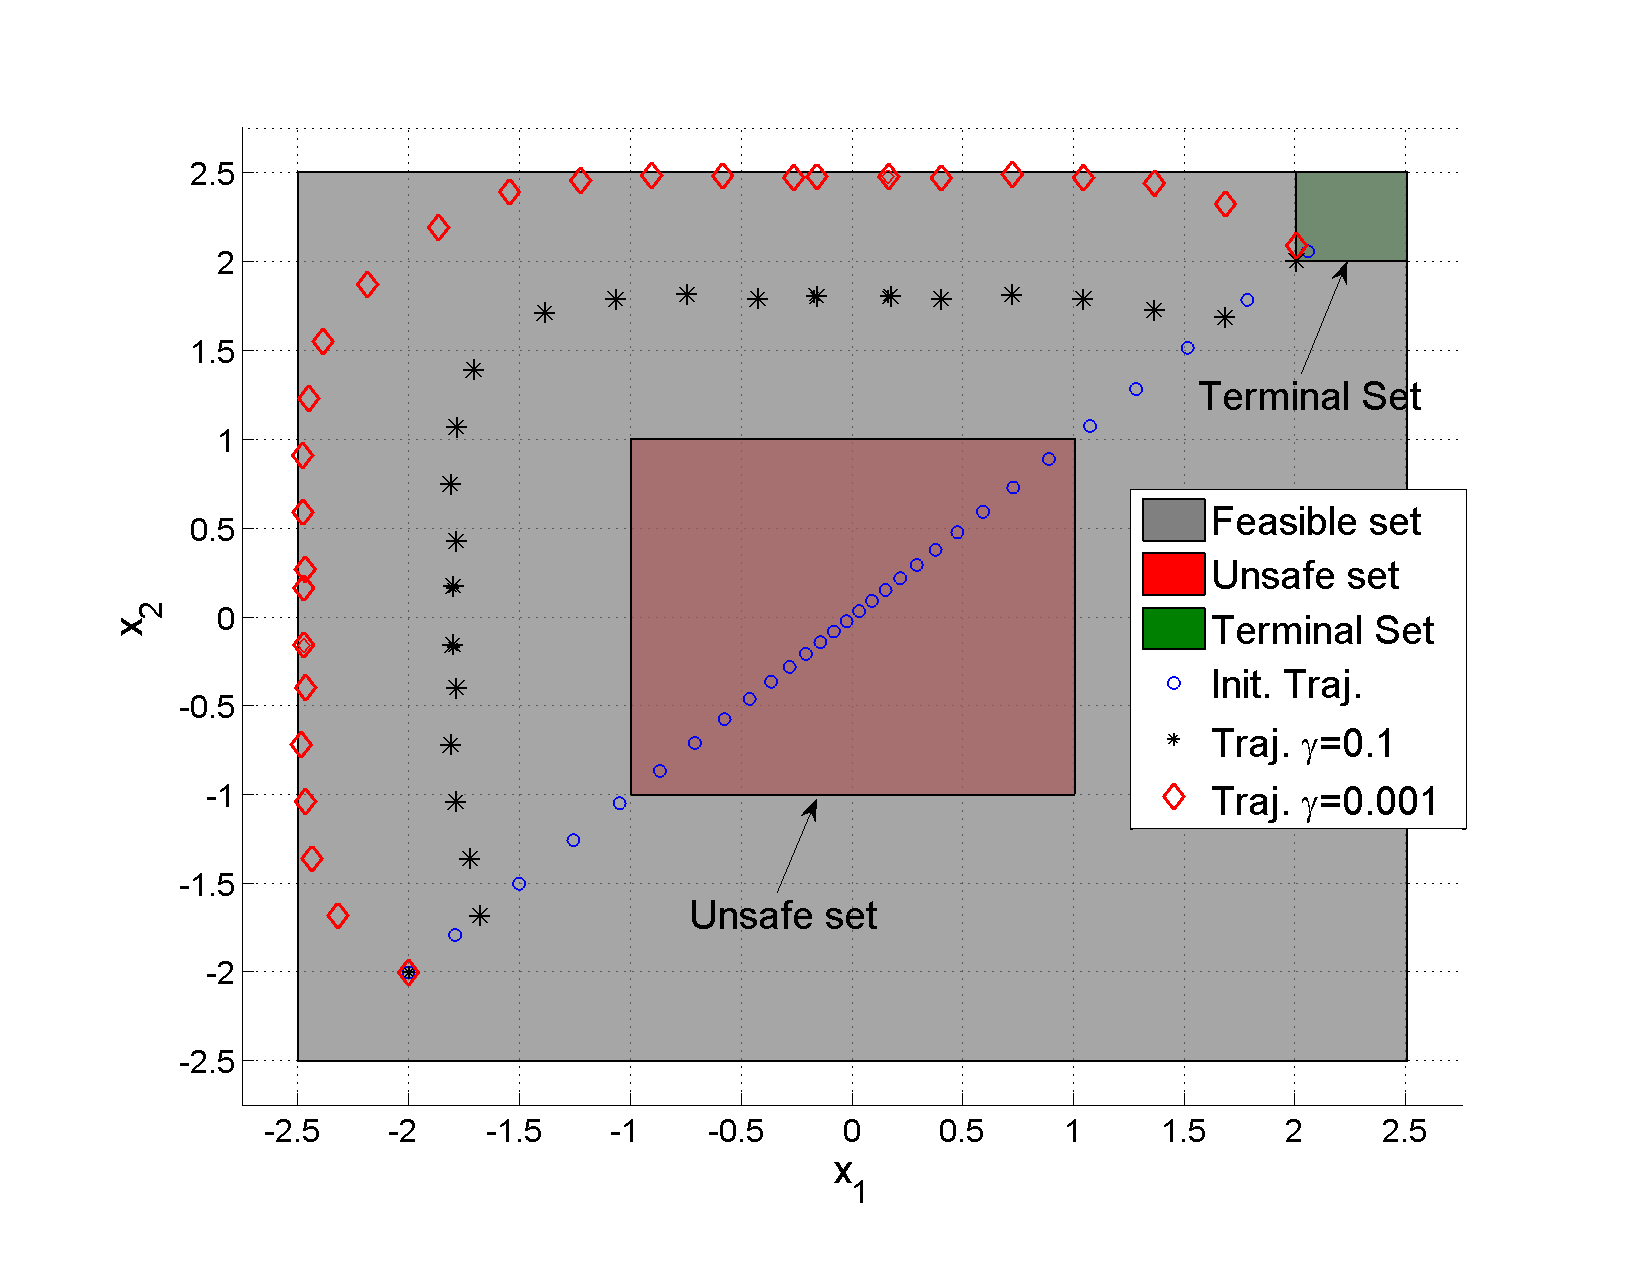
\includegraphics[width=0.49\textwidth]{figures/ToyExampleControl}
\caption{Initial trajectory and trajectories obtained for two different values of $\gamma$ in \eqref{eq:general_ctrl}.}
\label{fig:toy control}
\end{figure}

%% falsification example
%\subsection{Robustness minimization for falsification}
%\label{sec:toy falsification}
%Similar to the control problem, we can also minimize robustness to find trajectories that violate a given specification. Indeed, for the point-mass system, we solved such a problem ($\text{min}_{x_0 \in X_0} \, \srob(\sstraj) \, \text{s.t. } \sstraj=f(x_0,K)$) to find initial states such that the resulting trajectory, subject to a feedback controller $K$, violates a safety constraint. Our approach successfully finds such initial states, and so do gradient descent and simulated annealing on $\rob$. For brevity, we do not present these results here since all three methods result in the nearly the same solution, but note that our method can also be used to solve a falsification problem (\cite{AbbasATVA11_LinFalsification}, \cite{Deshmukh15_IterativeApproaches}).

%this blurb or the full example, pick your poisson:

%%Toy Falsification example



\begin{figure}[t]
\centering
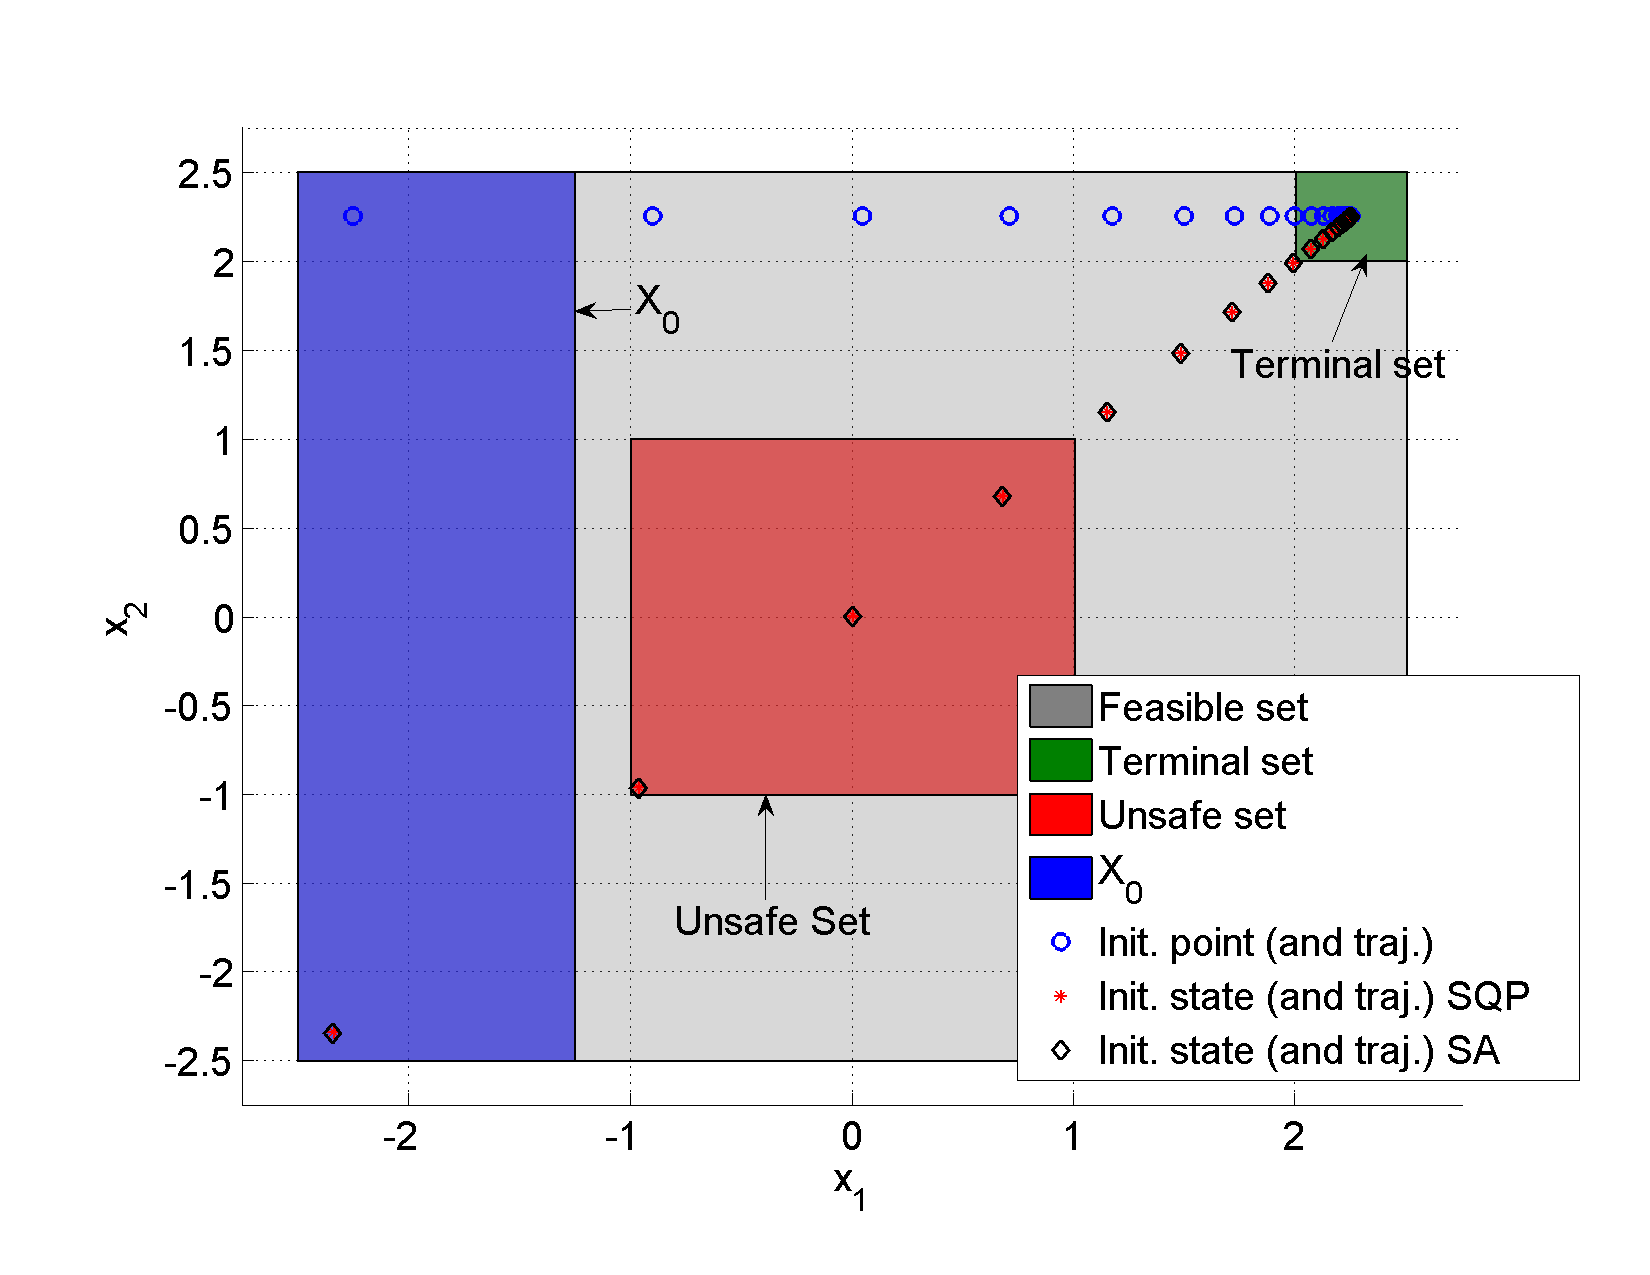
\includegraphics[width=0.49\textwidth]{figures/ToyExampleFalse}
\caption{Trajectories from initial points obtained from robustness minimization via Simulated Annealing (SA), SQP, and SQP on smooth robustness. Note, both SQP and SQP on smooth robustness lead to the same solution.}
\label{fig:toy falisification}
\end{figure}